% Chapter Template
\graphicspath{{/img}}
\chapter{Out-of-memory Graphics} \label{c3} % Main chapter title

Graphs are useful in statistics because it allows us to have a visual perspective of the data sets or to present them in a more meaningful way. However, when implementing graphics with survey data sets, it may become more difficult because the data sets are often large. For example, if every point of the large data set is plotted in a scatter plot, there will be too many points in the graph which will overlap and hide each other. There are two ways to over come this problem,

\begin{enumerate}
    \item Use different symbols, colour or sizes to represent different points or group of points. This is only suitable for data sets that are moderately large. If the data sets are too large, the points will still overlap each other.
    
    \item Condense multiple points into one point with an algorithm and use colours to represent the density of the sampling weights within the point. This will be discussed with more detail in section \ref{c3.3}.
\end{enumerate}

Another approach would be to take a sample from the full data set based on the estimated population distribution and plot the sample. \\

Currently, there are very few {\sf R} packages which allows us to plot graphs with data sets which are stored in a database. One of them is {\bf dbplot} \citep{dbplotpackage}, it is simple and light-weighted but it is in its early development stage. As for survey data sets, except for the {\bf sqlsurvey} package mentioned in section \ref{c1.1}, there are no packages that will allows us to plot data sets with sampling weights without having the data sets stored in memory.\\

Like the {\bf survey} package, {\bf svydb} also provides a set of tools for plotting survey data sets and is implemented with {\bf ggplot2} \citep{ggplotpackage}, but with less flexibility and options. Similar to the previous chapters, every graphical functions within {\bf svydb} is designed to do as much computation in the database as possible.

For some type of graphs, it is reasonable to produce them with data sets outside of memory, since to plot them, we don't need the whole data set in memory (computing the statistics for the graphs within the database may even be faster than transferring the whole data set into memory). For example, plotting a histogram with one variable, the only information that are needed to plot it is the location of the breaks for the x-axis and the density of the corresponding break for the y-axis. Say if there are 30 breaks, then at most we will only need 60 numbers in memory, 30 for the breaks and 30 for the density. 

An example of a graph that is not possible to plot without having the whole data set in memory is scatter plot, since we will need to know the location of all the points.

%----------------------------------------------------------------------------------------
\newpage
\section{Histogram} \label{c3.1}
Traditionally, the heights of each bin for a histogram while plotting the frequency, the height of each bin is determined by the number of values that are within the ranges of a certain bin, and plotting the density is determined by the proportion of data in each bin divided by the width of each bin.

To calculate the proportions, we first need to determine which bin each value is in. To do this we can use the {\ttfamily base::cut()} and perform {\ttfamily svydbmean()} on the cuts. However this function is not compatible with database tables, therefore a new function {\ttfamily db\_cut2} was implemented to overcome this difficulty, this will be discussed with more detail in section \ref{c3.1.3}.

\subsection{Usage} \label{c.3.1.1}
\begin{center}
    {\ttfamily svydbhist(x, design, binwidth = NULL, xlab = "x", ylab = "Density")}
\end{center}
\subsection{Arguments} 
\begin{itemize}
\item $x$ = Name indicating the variable.

\item $design$ = svydb.design object.

\item $binwidth$ = The width of each bin. Binswidths are calculated with Sturges' formula \citep{sturges} by default, $ k = [log_2 n] + 1$.}.
 
% Sturges, H. A. (1926). "The choice of a class interval". Journal of the American Statistical Association: 65–66. doi:10.1080/01621459.1926.10502161. JSTOR 2965501.

\item $xlab, ylab$ = labels for xlab and ylab.
\end{itemize}

\subsection{Examples} \label{c.3.1.2}
\begin{lstlisting}
> nh.dbsurv = svydbdesign(st = SDMVSTRA, wt = WTMEC2YR, 
    id = SDMVPSU, data = nhdb)
> svydbhist(x = DirectChol , design = nh.dbsurv,
    binwidth = 0.25)
\end{lstlisting}

\begin{figure}[h]
    \centering
    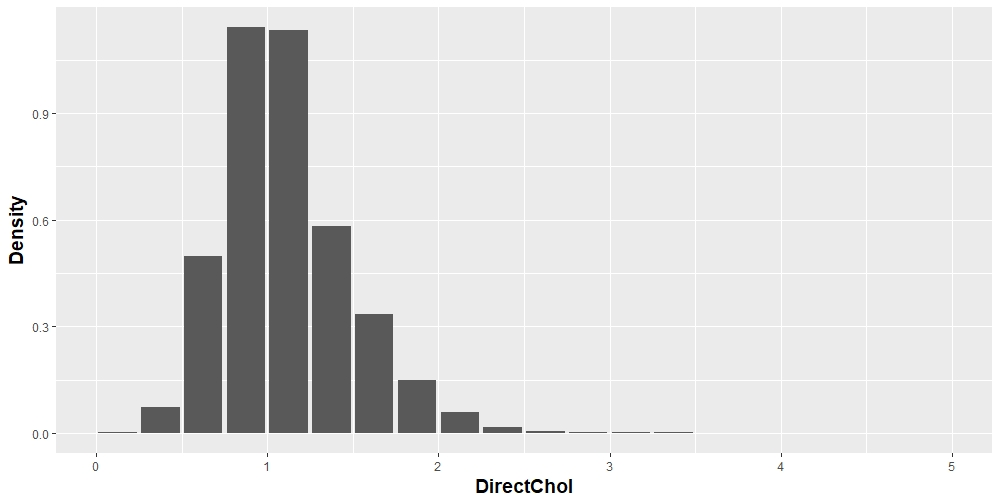
\includegraphics[scale = 0.55]{img/hist-e.jpeg}
    \caption{{\ttfamily svydbhist} example}
    \label{fig:hist-e}
\end{figure}




\subsection{Difficulty} \label{c3.1.3}
\begin{enumerate}
    \item In {\sf R}, it is simple to divide numeric columns into intervals by using {\ttfamily base::cut()}, but this function is not supported in {\sf SQL}. To overcome this problem a new function was written, {\ttfamily db\_cut2}, it is designed to be compatible with {\sf SQL} tables and is a simple version of {\ttfamily base::cut()}. 
\end{enumerate}

%----------------------------------------------------------------------------------------
\newpage
\section{Box Plot} \label{c3.2}

Boxplots are based on the quantiles of each variables or groups of variables. Traditionally, by default in {\sf R}, the boxes of the boxplot only uses the median, $25^{th}$ percent and $75^{th}$ percent quantile. The ends of the boxplots only extends out to the observations that are within the 1.5 $\times$ interquantile range, the rest of the observation outside this range are plotted as points. In {\ttfamily svydbboxplot} it is the opposite, due to efficiency.

\subsection{Usage} \label{c.3.1.1}
\begin{center}
    {\ttfamily svydbboxplot(x, groups = NULL, design, varwidth = F, outlier = F)}
\end{center}
\subsection{Arguments}
\begin{itemize}
\item $x, groups$ = If {\ttfamily groups} is defined, boxes of x will be split by {\ttfamily groups}.

\item $design$ = svydb.design object.

\item $varwidth$ = If {\ttfamily varwidth = T}, the width of the boxes will be proportional to the number of observations in that box.

\item $outlier$ = If {\ttfamily outlier = T}, Any observations above or below the $1.5IQR$ will be plotted as points.

\item $all.outlier$ = {\ttfamily TRUE} to plot all the outlier points, default {\ttfamily FALSE}.
\end{itemize}

\subsection{Examples} \label{c.3.1.2}
\begin{lstlisting}
> nh.dbsurv = svydbdesign(st = SDMVSTRA, wt = WTMEC2YR, 
    id = SDMVPSU, data = nhdb)
> svydbboxplot(x = Weight, groups = Race3, 
    design = nh.dbsurv, outlier = T, 
    all.outlier = F, varwidth = T)
\end{lstlisting}

\begin{figure}[h]
    \centering
    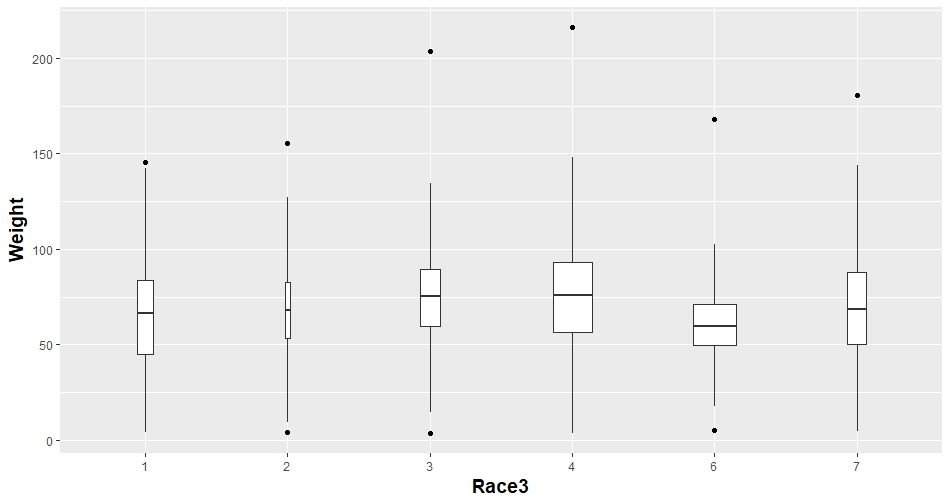
\includegraphics[scale = 0.55]{img/box-e.jpeg}
    \caption{{\ttfamily svydbboxplot} example}
    \label{fig:box-e}
\end{figure}

%----------------------------------------------------------------------------------------
\newpage
\section{Hexagon Binning} \label{c3.3}

As mentioned at the beginning of this chapter, since survey data sets can be large and scatter plots does not work well with large data sets because the points will hide or overlap each other. A solution would be to use hexagon binning \citep{hexbin}, group points that are close to each other into a hexagon and use colours or sizes of the hexagons to represent the sampling weights of all the points in every hexagon. The reasons of using hexagons will not be discussed here, but it is proven to be efficient and less biased visually. \\

Briefly, the hexagon binning algorithm works as follows, 
\begin{enumerate}
    \item Figure~\ref{fig:hex-e1} (Page~\pageref{fig:hex-e1}) Panel 1 - The red point represents the point to be binned. Blue and black point represents the dual lattice, each point represents the corner of each rectangle.
    
    \item Figure~\ref{fig:hex-e1} (Page~\pageref{fig:hex-e1}) Panel 2} - Figure out which rectangles are closest to the red point. The intersect of the two rectangles should contain the red point.
    
    \item Figure~\ref{fig:hex-e1} (Page~\pageref{fig:hex-e1}) Panel 3 - Figure out which hexagon the red point should be in by calculating the distance between the point and the centres of two hexagons. The centre for the blue hexagon is the top left corner of the black rectangle and the centre for the black hexagon is the bottom right corner of the blue rectangle.
    
    \item Repeat for the next point.
\end{enumerate}
%The algorithm repeats for every point.

\subsection{Usage/Arguments} \label{c.3.1.1}
To compute the hexagon bins:
\begin{center}
    {\ttfamily svydbhexbin(formula, design, xbins = 30, shape = 1)}
\end{center}

\begin{itemize}
\item $formula$ = A formula indicating x and y. i.e. y~x.

\item $design$ = svydb.design object.

\item $xbins$ = Number of bins on range of the x-axis.

\item $shape$ = plotting region, shape = height of y/width of x.
\end{itemize}

To plot the hexagon bins:
\begin{center}
    {\ttfamily svydbhexplot(d, xlab = d\$xlab, ylab = d\$ylab)}
\end{center}

\begin{itemize}
\item $d$ = returning object of {\ttfamily svydbhexbin()}.

\item $xlab, ylab$ = labels for x and y axis.
\end{itemize}

\newpage

\subsection{Examples} \label{c.3.1.2}
\begin{lstlisting}
> nh.dbsurv = svydbdesign(st = SDMVSTRA, wt = WTMEC2YR, 
    id = SDMVPSU, data = nhdb)
> hb = svydbhexbin(Height~Weight, design = nh.dbsurv)
> svydbhexplot(hb)
\end{lstlisting}


\begin{figure}[h]
    \centering
    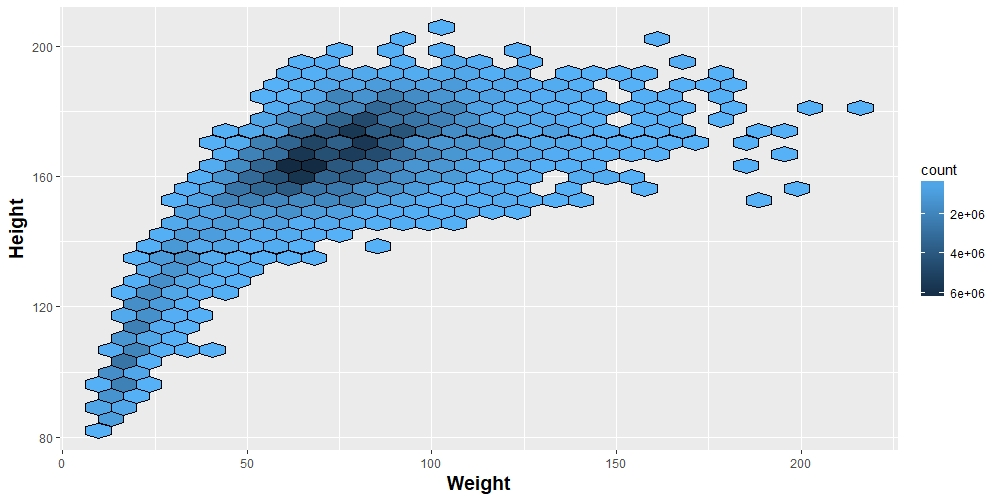
\includegraphics[scale = 0.55]{img/hex-e.jpeg}
    \caption{{\ttfamily svydbhexplot} example}
    \label{fig:hex-e}
\end{figure}

\subsection{Difficulties}

\begin{enumerate}
    \item The original code for hexagon binning in the {\bf hexbin} {\sf R} package \citep{hexbinpackage} used for-loops to run the algorithm, but it is not possible in {\sf SQL}. Therefore, new columns and extra calculations were needed to overcome this problem. This caused a efficiency problem.

\end{enumerate}

\begin{figure}[H]
\centering
    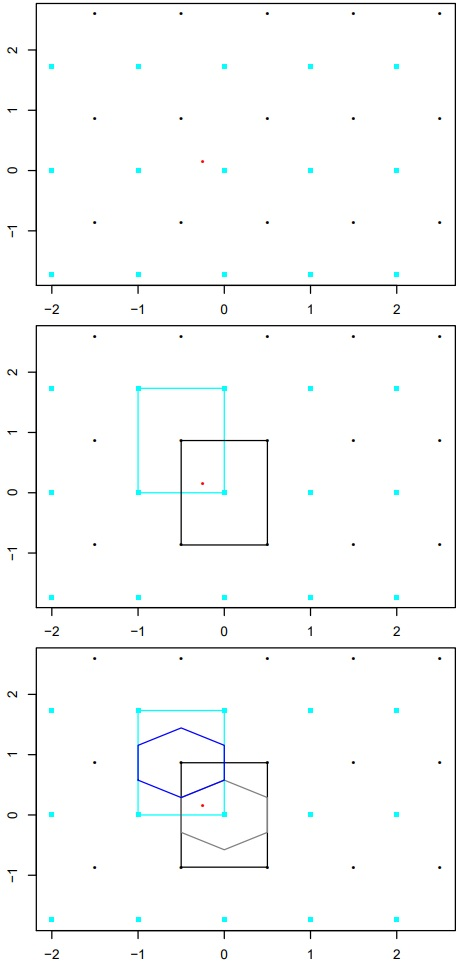
\includegraphics[scale = 0.9]{img/hex-e1.jpg}
    \caption{Hexagon binning explanation, \citep{hexbinfig}}
    \label{fig:hex-e1}
\end{figure}




%----------------------------------------------------------------------------------------
\newpage
\section{Conditional Plots} \label{c3.4}
% ref --- cleveland and co workers in the trellis display system
Conditional plots in {\bf svydb} products sets of hexagon binning graphs conditioned by the condition given by the user, both x and y axis will remain the same for all graphs. Currently it only supports conditions applied on factors.

\subsection{Function description} \label{c.3.1.1}
The {\ttfamily svydbcoplot()} function, has three basic arguments,
\begin{center}
    {\ttfamily svydbcoplot(formula, by, design)}
\end{center}

\begin{itemize}
\item $formula$ = Formula indicating x and y. i.e. y~x.

\item $by$ = Formula indicating the conditions of each plot. i.e by1~by2.

\item $design$ = svydb.design object.
\end{itemize}

\subsection{Examples} \label{c.3.1.2}
\begin{lstlisting}
> nh.dbsurv = svydbdesign(st = SDMVSTRA, wt = WTMEC2YR, 
    id = SDMVPSU, data = nhdb)
> svydbcoplot(Age~Height, by = SmokeNow~Gender, 
    design = nh.dbsurv)
\end{lstlisting}

\begin{figure}[h]
    \centering
    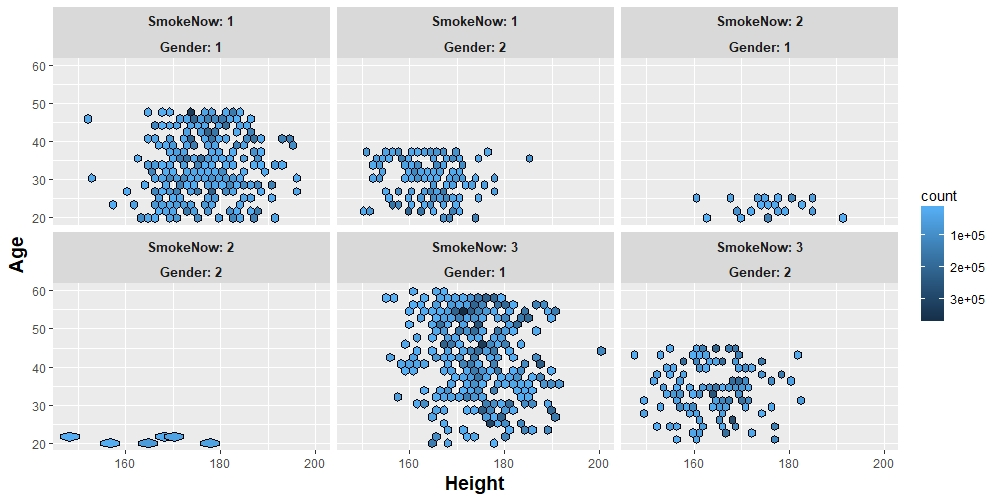
\includegraphics[scale = 0.55]{img/coplot-e.jpeg}
    \caption{{\ttfamily svydbcoplot} example}
    \label{fig:coplot-e}
\end{figure}
%----------------------------------------------------------------------------------------


\newpage
\section{Why ggplot?} \label{c3.5}

There are several reasons why  graphics in {\bf svydb} is implemented with {\bf ggplot2}, one of them is that {\bf ggplot2}, {\bf dplyr} and {\bf dbplyr} is maintained by the same group of people and is a part of a project at Rstudio. Though currently, {\bf ggplot2} is only compatible with data sets in memory, but it is possible this will change in the future. Another reason could be that the user would like to have a interactive plot, this done by {\bf plotly} \citep{plotlypackage}. \\

However, the main reason is that it provides more options for the users in terms of customising the plots. 
In base graphics, it would be difficult to customise plots when the arguments provided does not include what we want, also it would be difficult for the author to consider all the arguments when creating a function.\\

A simple example is that, when a {\ttfamily gg} or a {\ttfamily ggplot} object is created,
\begin{lstlisting}
> p = ggplot(mpg, aes(class, hwy))
\end{lstlisting}
Customising on the object is just as simple as adding other functions on,
\begin{lstlisting}
> p + geom_boxplot(varwidth = T) + 
    geom_jitter(width = 0.2) + coord_flip() + 
    ggtitle("plot") + theme_bw()
\end{lstlisting}

\begin{figure}[h]
    \centering
    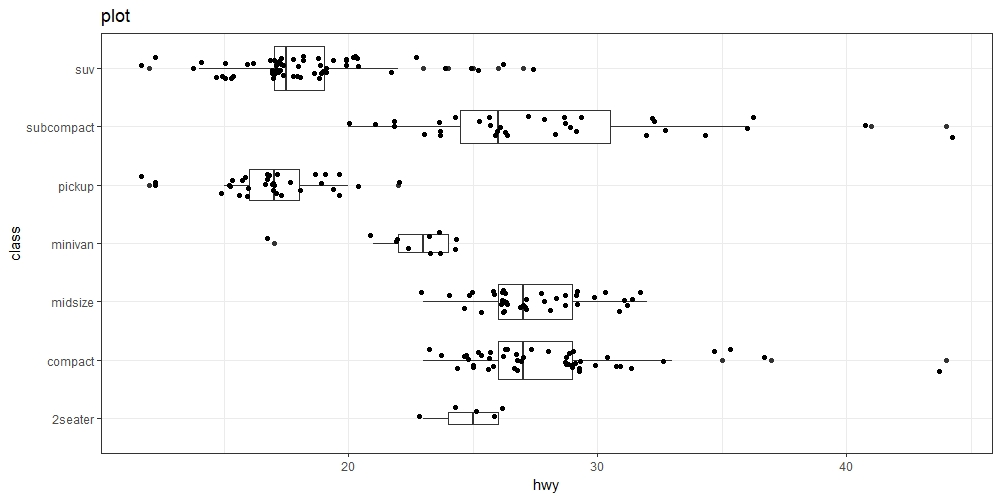
\includegraphics[scale = 0.55]{img/whygg1.jpeg}
    \caption{Why use {\ttfamily ggplot}}
\end{figure}

Or switching the style of the plot is as simple as changing the {\ttfamily geom},
\begin{lstlisting}
> p + geom_violin()
\end{lstlisting}

% \begin{figure}[h]
%     \centering
%     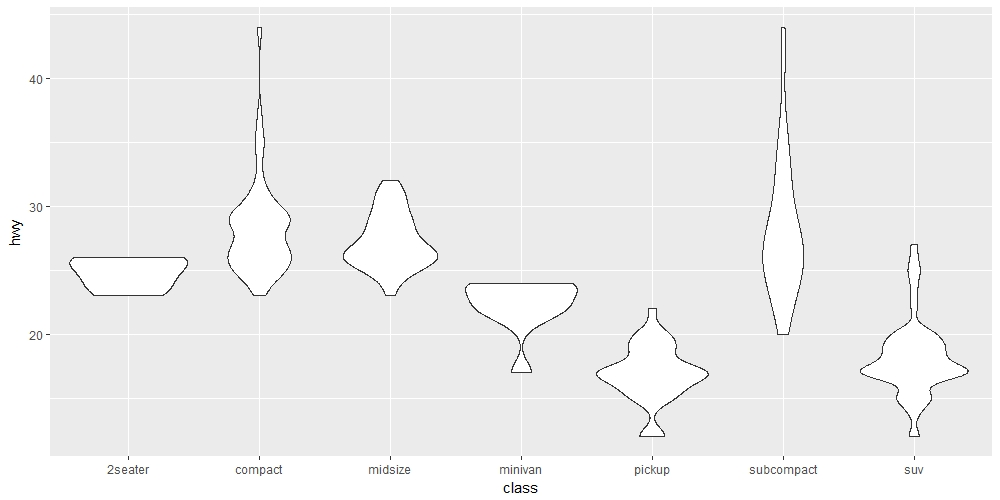
\includegraphics[scale = 0.55]{img/whygg2.jpeg}
% \end{figure}